\documentclass[12pt]{article}
\usepackage{geometry}                % See geometry.pdf to learn the layout options. There are lots.
\geometry{letterpaper}                   % ... or a4paper or a5paper or ... 
%\geometry{landscape}                % Activate for for rotated page geometry
\usepackage[parfill]{parskip}    % Activate to begin paragraphs with an empty line rather than an indent
\usepackage{daves,fancyhdr,natbib,graphicx,dcolumn,amsmath,lastpage,url}
\usepackage{amsmath,amssymb,epstopdf,longtable}
\usepackage{paralist}  % need to properly formulate standard answer blocks
\usepackage[final]{pdfpages}
\DeclareGraphicsRule{.tif}{png}{.png}{`convert #1 `dirname #1`/`basename #1 .tif`.png}
\pagestyle{fancy}
\lhead{CE 3305 Fluid Mechanics; Exercise Set 8}
\rhead{Name:\_\_\_\_\_\_\_\_\_\_\_\_\_\_\_\_\_\_\_\_\_\_\_\_\_\_\_\_\_\_\_\_\_\_}
\lfoot{REVISION A}
\cfoot{}
\rfoot{Page \thepage\ of \pageref{LastPage}}
\renewcommand\headrulewidth{0pt}
%%%%%%%%%%%%%%%%%%%%%%%%%%%%%%%%%%%%
\begin{document}
%%%%%%%%%%%%%%%%%%%%%%%%%%%%%%%%%%%
\begingroup
\begin{center}
{\textbf{{ CE 3305 Engineering Fluid Mechanics} \\ Exercise Set 8 \\ Summer 2018 -- GERMANY} }
\end{center}
\endgroup
\begingroup
~\newline
\textbf{Purpose} :  Application of concept of local acceleration in fluid flow to estimate pressure.\\
\textbf{Assessment Criteria} : Completion, plausible solutions, use \textbf{R} as a calculator. \\~\\
\textbf{Exercises}

\begin{enumerate}
\item (Problem 4.41 pg 160)
Water ($\rho = 1000 kg/m^3$) is accelerated from rest in a horizontal pipe that is 80 m long and 30 cm in diameter.  If the acceleration rate (toward the downstream end) is 5 m/s$^2$, what is the pressure at the upstream end if the pressure at the downstream end is 90 kPa gage? 


\item (Problem 4.49 pg 160)
Figure \ref{fig:Fountain} is a water jet issuing vertically from a nozzle   The water velocity as it exits the nozzle is 18 m/s.  Calculate how high $h$ the jet will rise.\footnote{Hint: Apply Bernoulli's equation along the centerline.}

\begin{figure}[htbp] %  figure placement: here, top, bottom, or page
   \centering
   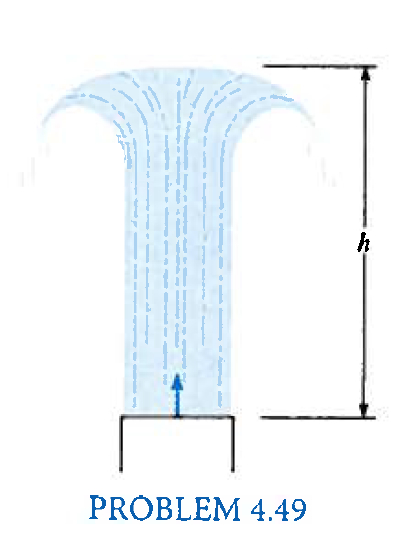
\includegraphics[width=2in]{Fountain.jpg} 
   \caption{Vertical jet fountain}
   \label{fig:Fountain}
\end{figure}

\end{enumerate}


\end{document}  